\documentclass{beamer}

\usefonttheme{professionalfonts} % using non standard fonts for beamer
\usefonttheme{serif} % default family is serif

\usepackage{hyperref}
%\usepackage{minted}
\usepackage{animate}
\usepackage{graphicx}
\def\Put(#1,#2)#3{\leavevmode\makebox(0,0){\put(#1,#2){#3}}}
\usepackage{colortbl}
\usepackage{tikz}
\usepackage{amssymb}
\usepackage{enumerate}
\usepackage{arydshln}
\usepackage{algorithm}
\usepackage{algpseudocode}

\colorlet{lightred}{red!25}
\colorlet{lightgreen}{green!25}
\beamertemplatenavigationsymbolsempty

\newcommand\blfootnote[1]{%
  \begingroup
  \renewcommand\thefootnote{}\footnote{#1}%
  \addtocounter{footnote}{-1}%
  \endgroup
}

\makeatletter

%% Textclass specific LaTeX commands.
\newcommand\makebeamertitle{\frame{\maketitle}}%
\AtBeginDocument{%
  \let\origtableofcontents=\tableofcontents
  \def\tableofcontents{\@ifnextchar[{\origtableofcontents}{\gobbletableofcontents}}
  \def\gobbletableofcontents#1{\origtableofcontents}
}
%% User specified LaTeX commands.
\usetheme{Malmoe}
\useoutertheme{infolines}
\addtobeamertemplate{headline}{}{\vskip2pt}
\setbeamercovered{transparent}

\makeatother

%%%%%%%%%%%%%%%%%%%%%%%%%%%%%%%%%%%%%%
%% Main document
%%%%%%%%%%%%%%%%%%%%%%%%%%%%%%%%%%%%%%
\begin{document}
\title[PFLOCK report]{PFLOCK Report}
\author[AC]{Andres Calderon}
\institute[Spring'20]{University of California, Riverside}
\makebeamertitle
\newif\iflattersubsect

\AtBeginSection[] {
    \begin{frame}<beamer>
    \frametitle{Outline} 
    \tableofcontents[currentsection]  
    \end{frame}
    \lattersubsectfalse
}

\AtBeginSubsection[] {
    \begin{frame}<beamer>
    \frametitle{Outline} 
    \tableofcontents[currentsubsection]  
    \end{frame}
}

\begin{frame}{Experiment settings}
  \begin{itemize}
    \item Working with the new Quadtree implementation.
    \item Varying a value to limit the size of the cell. It was between 1 and 5 times the $\varepsilon$ value.
    \item Varying the number of partitions between 8 and 12 times the number of available cores (108).
    \item Finding disks for LA50K dataset using $\varepsilon$ 10m.
    \item Using 12 nodes with 9 cores each.
    \item Collecting the task with longest duration for each case. Average of 5 runs.
  \end{itemize}
\end{frame}

\begin{frame}{Results}
  \centering
  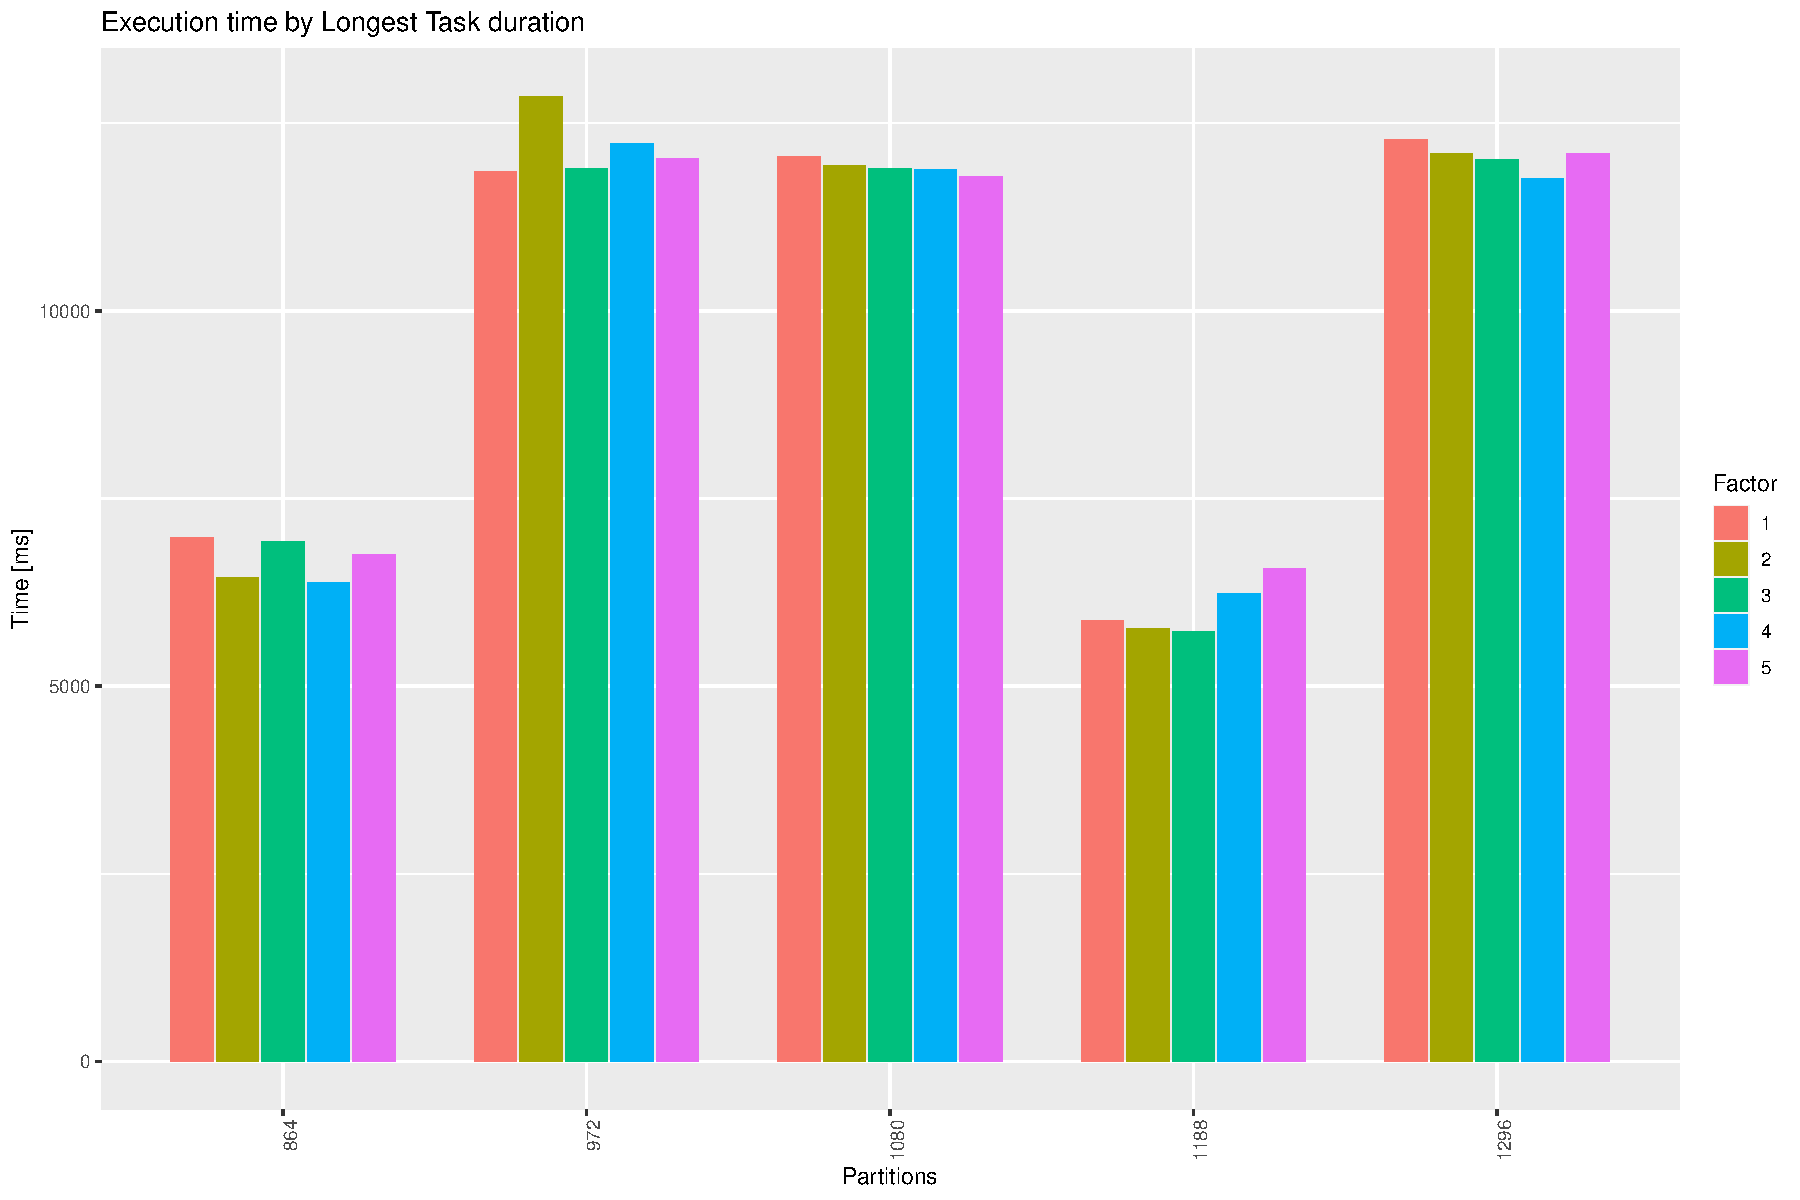
\includegraphics[width=\textwidth]{figures/TopTaskDuartion}
\end{frame}

\begin{frame}{Results}
  \centering
  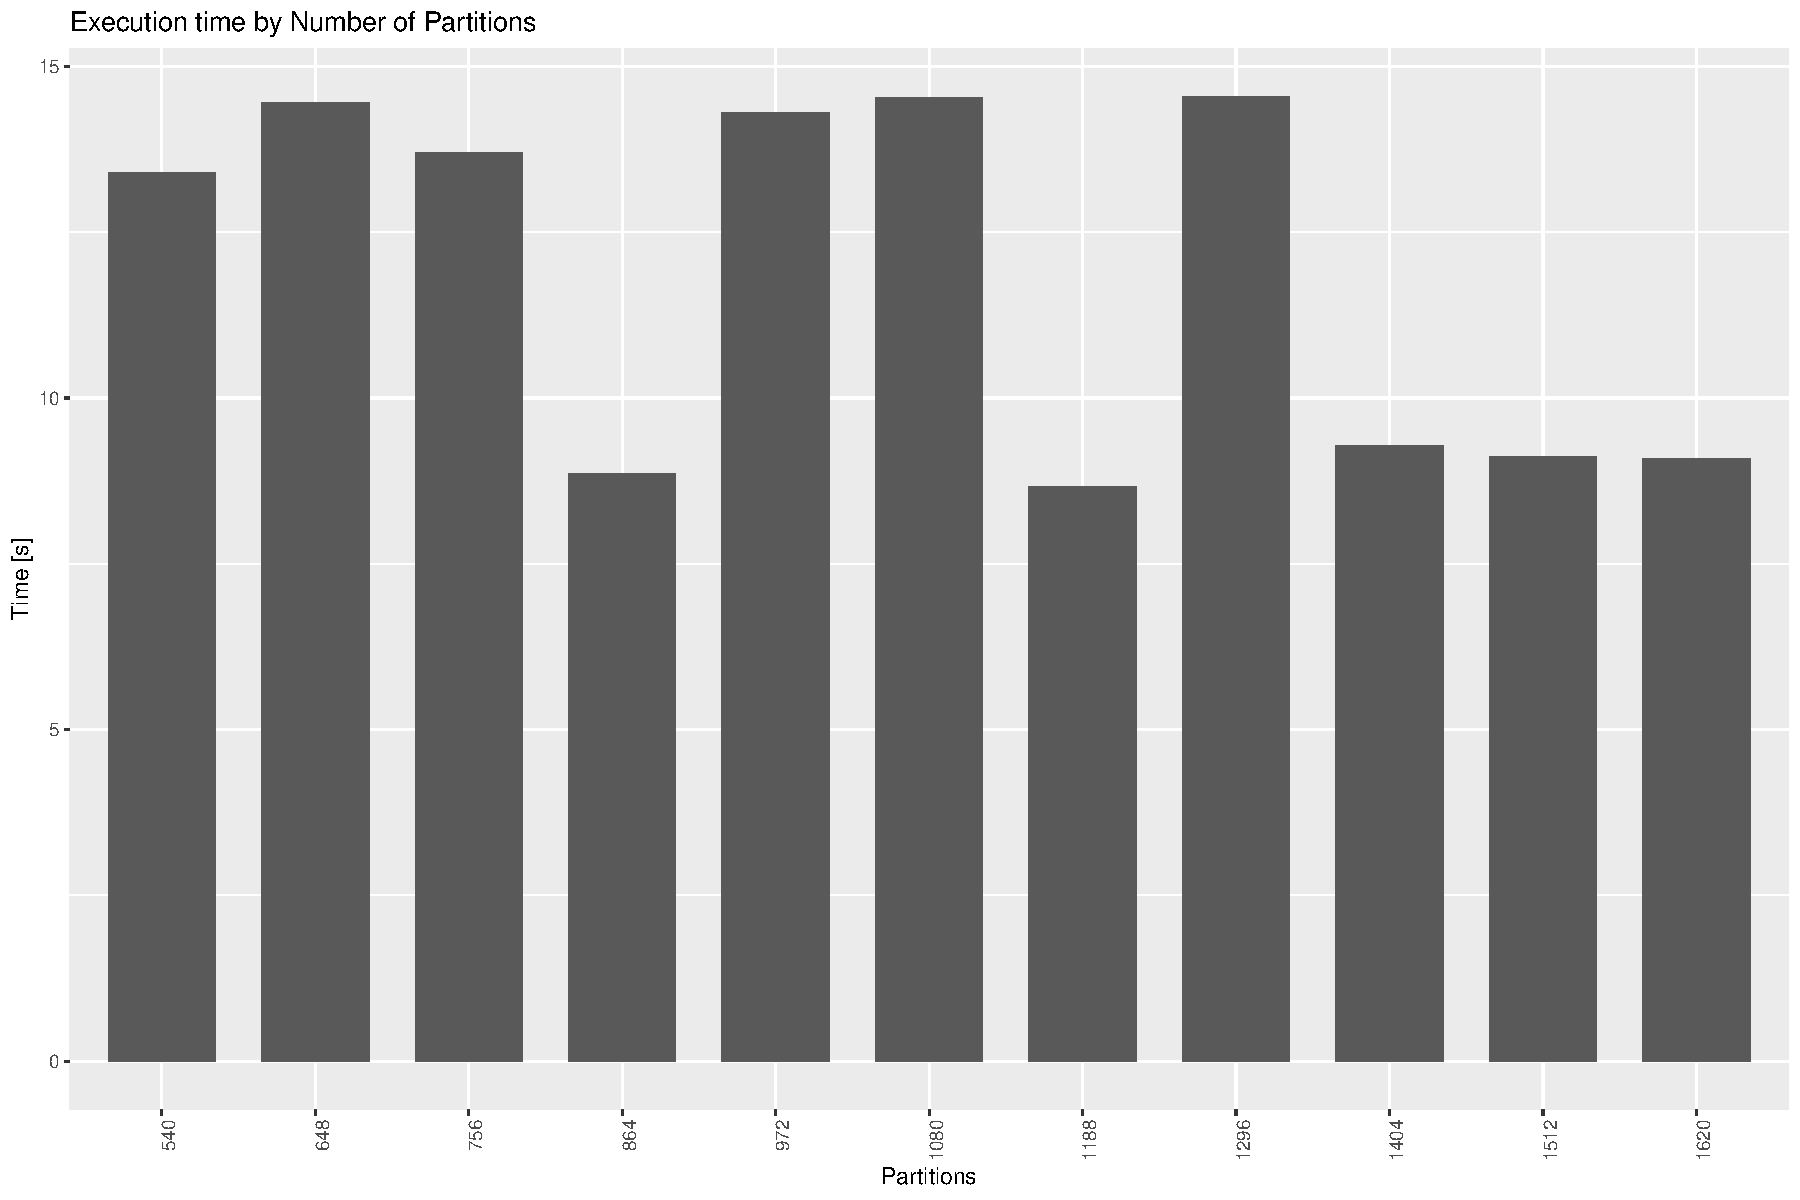
\includegraphics[width=\textwidth]{figures/ByPartitions}
\end{frame}

\begin{frame}{What's next}
    \begin{itemize}
        \item Check the distribution of partitions of longest tasks to confirm behaviour.
        \item Double-check with previous implementation.
        \item Give a try with a different dataset.
    \end{itemize}
\end{frame}

\end{document}

